As discussed in the DQN (section 3.2), the best result we had for this approach was a 2 conv-nets followed by two linear layers with appropriate dimensions model, trained with three images at a time (current images and past two). On top of that, the usual "tricks" to make it work better were used, like experience replaly and delayed target network for more stability in training and for more data efficiency, and, arguably most important, a carefully tuned $\epsilon$, capping it $0.3$ and training like that for many time-steps before annealing it further. \\


\medskip
\noindent
The plots were computed with saves of the model on every 1000 episode, setting the $\epsilon=0$ (setting the model completely greedy wrt. the $Q$ action-value function during the test). As explained in section 3.2, the model had $\epsilon$ annealed from 1 to 0.3 during the first tens of thousands of episode, then capped at $\epsilon=0.3$ until 125000 and then annealed further until $0.1$, capping it there around episode 160000.

\medskip
\noindent
It seemed that the model easily overfitted it's high values to it's already seen winning action-states when $\epsilon$ was annealed to low values of $0.1$ before it got good enough. Capping $\epsilon=0.3$ for a much longer period of time lead to having enough exploration, generalized well enough and was able to further improve.


\begin{figure}[ht!]
    \centering
    \begin{subfigure}{0.49\textwidth}
        \centering
        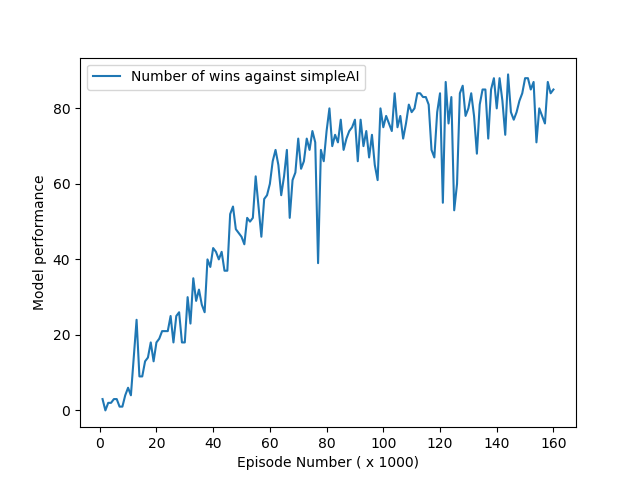
\includegraphics[scale=0.4]{figures/dqn_results_wins.png}
        \caption{Number of wins}
        \label{fig:Number of wins}
    \end{subfigure}
    \begin{subfigure}{0.49\textwidth}
        \centering
        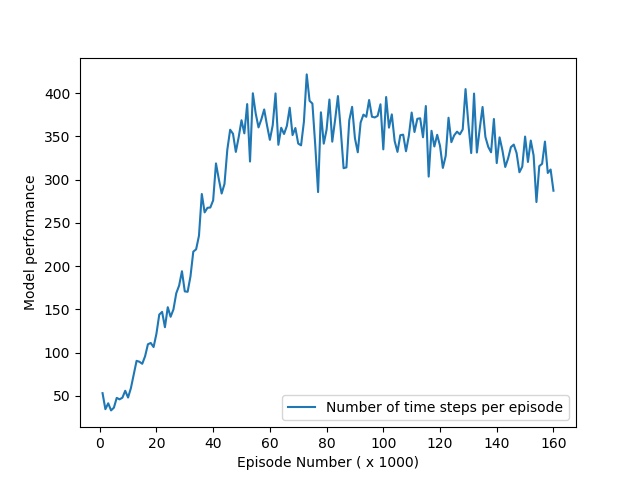
\includegraphics[scale=0.4]{figures/ttd_per_episode.png}
        \caption{ Average timesteps being alive for during episodes}
        \label{fig: Average timesteps being alive for during episodes}
	\end{subfigure}    
    \caption{Average timesteps and wins against simpleAI}
\end{figure}

\begin{figure}[ht!]
    \centering
    \begin{subfigure}{0.49\textwidth}
        \centering
        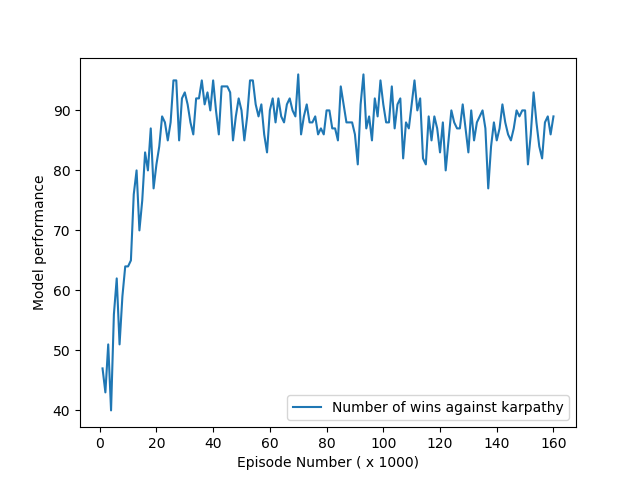
\includegraphics[scale=0.4]{figures/dqn_results_wins_vs_karpathy.png}
        \caption{Number of wins}
        \label{fig:Number of wins}
    \end{subfigure}
    \begin{subfigure}{0.49\textwidth}
        \centering
        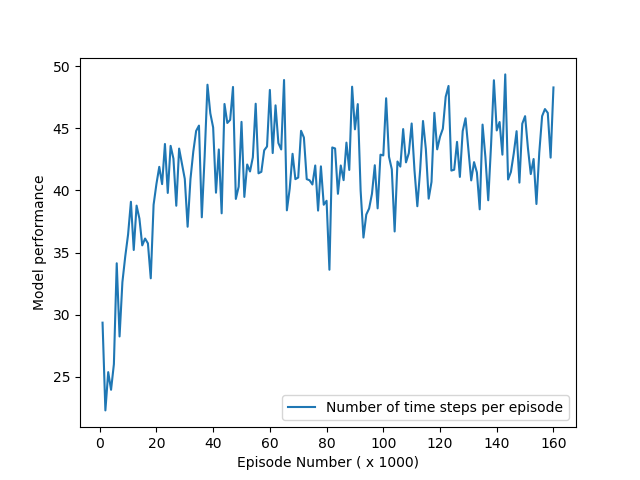
\includegraphics[scale=0.4]{figures/ttd_per_episode_vs_karpathy.png}
        \caption{ Average timesteps being alive for during episodes}
        \label{fig: Average timesteps being alive for during episodes}
	\end{subfigure}    
    \caption{Average timesteps and wins against Karpathy}
\end{figure}
 

\begin{figure}[ht!]
	\centering
	\begin{subfigure}{0.49\textwidth}
        \centering
        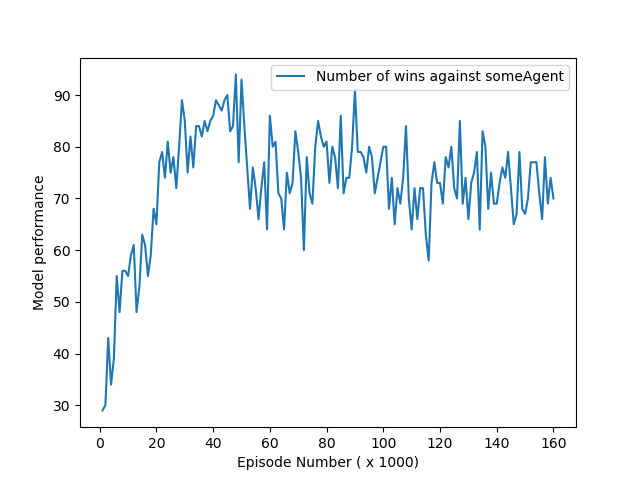
\includegraphics[scale=0.4]{figures/dqn_results_wins_vs_someagent.png}
        \caption{Number of wins}
        \label{fig:Number of wins}
    \end{subfigure}
    \begin{subfigure}{0.49\textwidth}
        \centering
        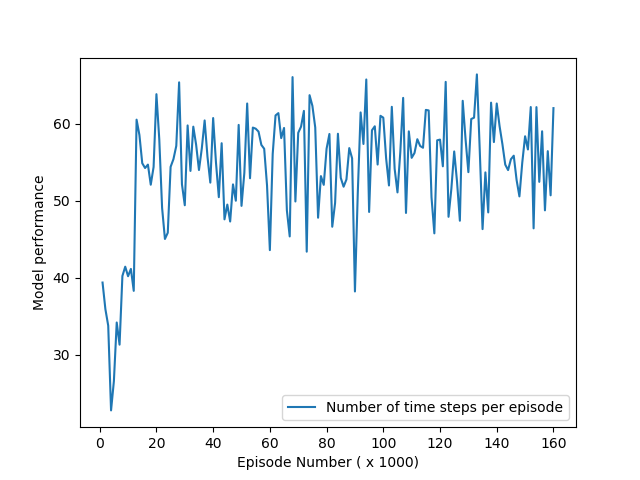
\includegraphics[scale=0.4]{figures/ttd_per_episode_vs_someagent.png}
        \caption{ Average timesteps being alive for during episodes}
        \label{fig: Average timesteps being alive for during episodes}
	\end{subfigure}    
    \caption{Average timesteps and wins against Someagent}
\end{figure}

\pagebreak

\medskip
\noindent
Figure 4 shows the results versus a completely random model. Before blacking out the right pannel in the training images, we were only getting about 50\% win-rate versus this completely random model. That gave us the hint that the model is actually overfitting ($Q$ action-value function was predicting values more on the position of the right pallet rather it's own pallet relative to the ball). This, along with rendering the model helped us realise the model was not at all generalizing and it learned to just imitate simpleAI.
